\section{Image Reconstruction with Compressed Sensing} \label{cs}
The push to wide Field of View imaging has led to increased research into Compressed Sensing. 



The flexibility allows for a lot of freedom in design which can lead to different approaches for the same problem. So far, there are no 'best practices' for Astronomy: No prior, objective or optimization algorithm works strictly better than every other choice. Furthermore the choices for the individual parts influence each other. Compressed Sensing is flexible, but not every optimization algorithm works with every prior.

%In this project, the GuRoBi optimization algorithm was used. It uses the Simplex to solve the quadratic programming problems. It  out to be not ideal for the Inverse Problems of Radio Astronomy. However

%Idea behind compressed sensing

\subsection{The Sparseland Prior and Incoherence: How Compressed Sensing works}
For Compressed Sensing we need a Prior $P$ in which our signal can be sparsely represented. It is not guaranteed that such a space exists, but for natural signals there always seem to be. This has led to the idea of the Sparseland Prior \eqref{cs:eq:sparseDic} which is at the core of Compressed Sensing: We assume for our signal $x$ there exists a dictionary $D$. Each entry represents a signal part which can be present. $D$ is potentially a large, but has a finite number entries. We assume that any $x$ can only consist of a few signal parts of $D$. This means the coefficients for the signal parts in the dictionary $\alpha$ are all zero except for $s$ entries for all valid $x$. 

\begin{equation} \label{cs:eq:sparseDic}
	\begin{split}
		x = D \alpha  \qquad  x \in \mathbb{R}^{n}, \alpha \in \mathbb{R}^{m}, D \in \mathbb{R}^{n*m}, \qquad n \leq m \\
		\left \| \alpha \right \|_0 = s \qquad s \ll n \leq m
	\end{split}
\end{equation}

In image compression this phenomenon was can already be observed: image depicting nature scenes tend to be sparse in the wavelet domain. If $x$ in \eqref{cs:eq:sparseDic} are nature scenes, we can create a Dictionary $D$ of wavelets. A single image $x$ can be represented with a few wavelets, meaning the number of non-zero entries $s$ in $\alpha$ is far lower than the number of pixels $n$. All that is left to do for compression is save the non-zero entries of $\alpha$. Two effects are of note: When $x$ is noisy, or when $x$ is not a nature image, the resulting $\alpha$ is not sparse. In Compressed Sensing this fact is exploited to reconstruct the true image from under-sampled measurements.

%So when we use a camera to make a picture of a nature scene, the camera produces megabytes of data which all get compressed to a handful of kilobytes before they are saved to a disk. The compressed image is accurate enough that a human eye cannot distinguish it from the raw image. Which leads to the question: If only a handful of kilobyte are needed, can we somehow only measure the needed data? The Nyquist-Shannon sampling theorem states that this is not possible: If we sample below the Nyquist Shannon rate, there are many possible images that fit the measurement and we cannot distinguish which is the right one. With Compressed Sensing we can do exactly that: Because we know our image is sparse in the wavelet domain, we can use it to determine which of the many possible image is true.

Back to the ill-posed inverse problem of interferometry: We measure the complex Visibilities of a band-limited signal. The Nyquist-Shannon rate states that if our band limited signal has at most frequency $f$, our sample frequency needs to be higher than $2f$. For $n$ pixels, this is the case when we measure all $n$ complex Visibilites (two samples per Visibility). If we have fewer samples, the Nyquist Shannon theorem states we cannot reconstruct the true image.

But what if we know our image is a Sparseland Signal and we happen to know the dictionary? Let us assume our image consists of $n = 20*20$ pixels and our dictionary of $m = 1000$ wavelets. Further assume at most $s=10$ of the wavelets are non-zero for a given image. Could one just measure the 10 non-zero components of $\alpha$ and reconstruct the image? If we have prior knowledge about the location of the non-zero components, we would need 10 samples to reconstruct the image. Sadly, this is not the case in general. With the first sample we have about a $1/100$ chance of measuring a non-zero component. Note that if we measure a non-zero component, we learn $1/10$ of the information about the image. If we hit a zero component, we learn practically nothing. The question is, is there a way we can maximize our information gain of the non-zero components for each sample? In fact, there is: By having the measurement space be  as incoherent as possible from the dictionary space, we maximize the information gained per sample.

[How many samples are needed]

Constructing an incoherent sampling space is surprisingly easy. Random projections are likely to produce a incoherent sampling space. Since we use an interferometer, we are bound to measure in Fourier Space. Depending on the prior, the Fourier Space might be coherent with the dictionary space and we do gain the maximum amount of information. As discussed in section \ref{radio}, wide Field of View imaging breaks the two dimensional Fourier relationship. McEwen et al\cite{mcewen2011compressed} showed that the wide Field of View measurement equation can help with incoherence, and demonstrated higher image reconstruction quality on simulated data.

The Sparseland prior is the basis of which Compressed Sensing builds. The dictionary can contain any function and is not limited to wavelets. It can even contain a mixture of for example wavelets, gaussians and cosine functions. Sparseland priors lend themselves to over-complete representations, where the number of dictionary entries is multiple times higher than the number of pixels($m \gg n$). 

An appropriate prior for Radio Astronomy is still under research, currently Starlets\cite{starck2015starlet} and Curvelets\cite{starck2003astronomical} are on top of the foodchain


\subsection{Objective Function}
The Compressed Sensing CLEAN objective function \eqref{intro:eq:csclean} uses the L0 norm for it's regularization term, which means the Objective Function is not convex. There are specialized solvers for the L0 compressed sensing. The L1 relaxation however is practically guaranteed to have the same minimum as the L0 norm and results in a convex objective function. Since GuRoBi works better on the L1 relaxation it was chosen for this project.

There are three different Compressed Sensing objectives: The analysis method, where the image $x$ is minimized directly, the synthesis method where the sparse vector $\alpha$ is minimized, or by in-painting the missing Visibilities $V_2$.

\begin{alignat*}{2}
	analysis:\qquad \underset{x}{minimize} \:& \left \| D_{dirty} - x \star PSF \right \|_2^2 &&+  \lambda \left \| Px \right \|_1 \\
	synthesis:\qquad \underset{\alpha}{minimize} \:& \left \| D_{dirty} - D \alpha \star PSF \right \|_2^2 &&+ \lambda \left \| \alpha \right \|_1 \\
	in-painting:\qquad \underset{V_2}{minimize} \:& \left \|  D_{dirty} - F^{-1} M V_2 \right \|_2^2 &&+ \lambda \left \| PF^{-1}V_2\right \|_1
\end{alignat*}

All three objective functions have the same global minimum. Retrieving $x$ for the analysis objective is trivial, or the second and third objective $x$ can be retrieved by $x = D\alpha$ and by $x = F^{-1}V_2$ respectively. [Empirical and theoretical studies have shown an advantage of the analysis objective over the other two \cite{something}]. However, depending on the measurement space, prior and optimization algorithm, one objective may be easier to solve than others. The analysis objective is not useful when there is no transformation from $x$ into the sparse space. This is the case for most over-complete priors: In that case, $P$ is a $m*n$ matrix and  $Px \ne \alpha$. The synthesis method just requires a transformation from the sparse space to image $D\alpha = x$. Similarly one might chose the in-painting method when the prior is a convolution in image space: Convolutions in image space are equivalent to a multiplication in Fourier Space.

wide field imaging considerations
\begin{equation}\label{cs:eq:wfield}
	\underset{x}{minimize} \: \left \| V - MF_{WFOV} x \right \|_2^2 + \lambda \left \| Px\right \|_1
\end{equation}

%How to setup $F_{FOV}$. It is in the easiest case. Often, V is sampled on a regular Grid an A can the A-projection matrix
A-projection lofar \cite{tasse2013applying}


%A lot of freedom to choose. For this project CASA was used, which limits the choices.

\subsection{Compressed Sensing Algorithms in Astronomy}



\subsubsection{SASIR}
Prior: Starlets

Objective: in-painting

Optimizer: FISTA


\subsubsection{PURIFY}
Prior: Mixture of Dirac functions and Daubechies wavelet (DB1 - DB8)

Objective: analysis

Optimizer: SDMM

Dirac is a fancy way of saying "it is sparse in pixel space"


\subsubsection{Vis-CS}
Prior: dictionary of gaussians

Objective: Synthesis

Optimizer: Coordinate descent

\pagebreak
\subsubsection{Implementation In Casa}

\begin{wrapfigure}{r}{0.6\textwidth}
	\centering
	\vspace{-15pt}
	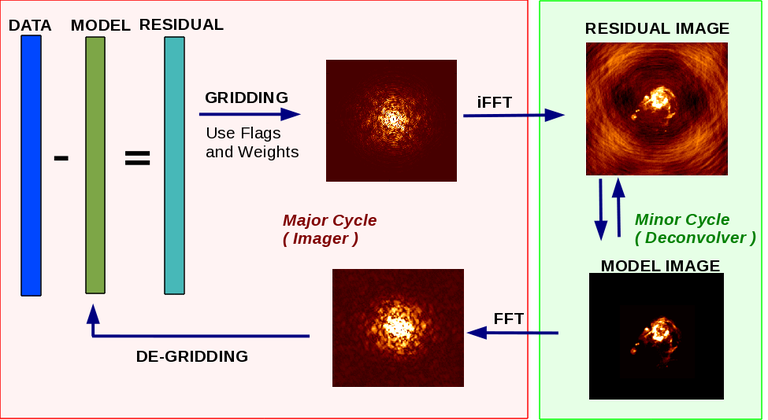
\includegraphics[width=0.9\linewidth]{./chapters/04.cs/img/casa_major_minor.png}
	\caption{Casa Major Minor Cycle, source \cite{casa2018major}}
	\label{cs:major}
	\vspace{-10pt}
\end{wrapfigure}

Terminology in CASA.

CASA is a software package built for solving the deconvolution problem for instruments like VLA and ALMA. "Data" Column measurements(calibrated), model column contains the "true" visibilities and the residual column only noise. The architecture is oriented after the CLEAN algorithm, it is split in a major and minor cycle.\ref{cs:major}. The first part of the major cycle produces the dirty image and the PSF. The minor cycle is where a deconvolution algorithm "cleans" the dirty image, several iterations of CLEAN. Major cycle ends with the forward fourier transform. Chi$^2$ approximation of the visibilities. At the end of several major cycle, the Model column should contain an approximation of the true visibilities while the Residuals should be pure noise.

Wide field of view imaging aka A- and W- Projections are handled in the major cycle.  most often a CLEAN derivate.

\begin{figure}
		\centering
		
		\caption{Restoration Process in CASA}
		\label{cs:restoreimage}
\end{figure}

Dirty image, Model image and cleaned image

The idea of the dirty beam and the clean beam. The output of CASA is the model image convolved with the clean beam plus residuals. Because the model image contains many small peaks, any structure smaller than the clean beam is implausible. Convolving with a gaussian is essentially reducing the resolution. But this is not the case. CLEAN can lead to implausible model images depending on the content: If only a few point sources are visible, clean is plausibe. But for extended emissions clean produces a an area of many peaks which is not true.. With compressed sensing, the ideal prior leads to the true model image. 

CASA can be extended new deconvolution algorithms, changing minor cycles. During the project it was evaluated if CASA could be modified so wide Field of View imaging can handled by the minor cycle. It was not possible. The implementation is restricted to the deconvolution in the data term. This excludes the in-painting objective function. Or that the data term minimizes on the Visibilities directly.




 
